%\addcontentsline{toc}{chapter}{Development Process}
\chapter{Design}

\section{Overall Architecture}\label{arch}

The overall architecture of the system can be described as a mixture of two well known architectural patterns, Model View Controller(MVC) and 3-tier architecture. 

\subsection{MVC}\label{sec_mvc}

The Model View Controller paradigm is synonymous with web application development these days and is often employed without much consideration for alternatives. The fact is that the MVC pattern is so ubiquitous and well supported and understood that it is difficult to make a case against its use for a project of this nature, where MVC fulfils all expectations for a data driven front end to a web application. Many of the alternative approaches share the same primary goal as MVC, seperation of concerns, keeping the display and data components separate. However these alternatives lack the penetration that MVC currently has and as such their comparative obscurity makes them less desirable from a general maintenance point of view since it can be expected that a greater number of developers will already be familiar with MVC. Many mature and well maintained frameworks offer MVC as default out of the box in a well supported and easy to understand manner, for these reasons not much consideration was given to other possible solutions although some were briefly looked at.

Figure~\ref{fig:mvc} provides a high level overview of the way in which the MVC pattern is structured. For this project, each web page will be represented as its own view with its own dedicated controller, providing a high degree of modularity and helping to keep the individual controller classes thin in order to aid code navigation, maintainability and scalability of the solution. 

\begin{figure}[H]
    \centering
    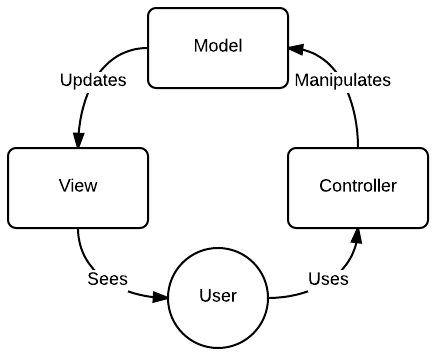
\includegraphics[width=0.5\textwidth]{images/design/mvc}
    \caption{Model View Controller pattern overview}
    \label{fig:mvc}
\end{figure}


\subsection{3-tier Architecture}
The second architecture pattern making up the system design is 3-tier architecture. The goal of the 3-tier pattern is to separate the system into 3 distinct, modular tiers. These layers are the presentation layer, the business logic or service layer and the persistence layer.  

In this project the presentation tier encapsulates the entirety of MVC pattern described in section~\ref{sec_mvc} above, the MVC controller for a particular view will make a request to a service layer class and use the resulting data to populate a model for returning to the view.

 The service layer is where the business processes are carried out. Logical processes, data transformations and calculations are all carried out within this tier. The service layer also acts as a go-between for the presentation and persistence layer, translating requests and results into compatible forms for the other tiers.
 
 The persistence layer, or data layer, is concerned with data storage and retrieval, usually, and for this project entirely, from a database system. All crud operations and queries on database entities are performed within this layer allowing the service layer and its containing logic to be abstracted away from the database.
\begin{figure}[H]
    \centering
    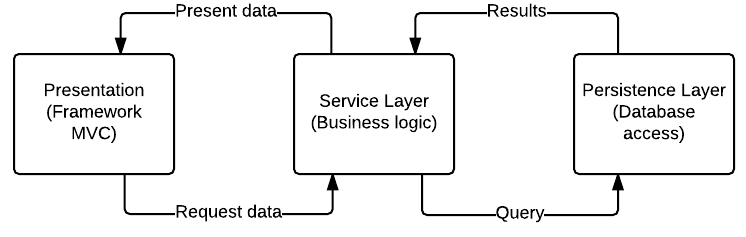
\includegraphics[width=\textwidth]{images/design/3t}
    \caption{3-tier architecture overview}
    \label{fig:3t}
\end{figure}

The 3-tier pattern is a useful design within this project because it allows modularised and compartmentalised code to be written and maintained. Using the 3-tier pattern allows a developer to modify one of the distinct layers without having to rewrite the entire system. For example, all the queries and database calling methods could be changed to use totally different technologies and provided the same hooks are available for the service layer to gain access then the system would function as expected with no modification to service or presentation layers. Figure~\ref{fig:arch1} shows the relationship between layers using a subset of the system components. Service layer dependencies are wired into each controller that require access to the processes in that service or the data in the database access object (Dao) coupled to a given service. 

\begin{figure}[H]
    \centering
    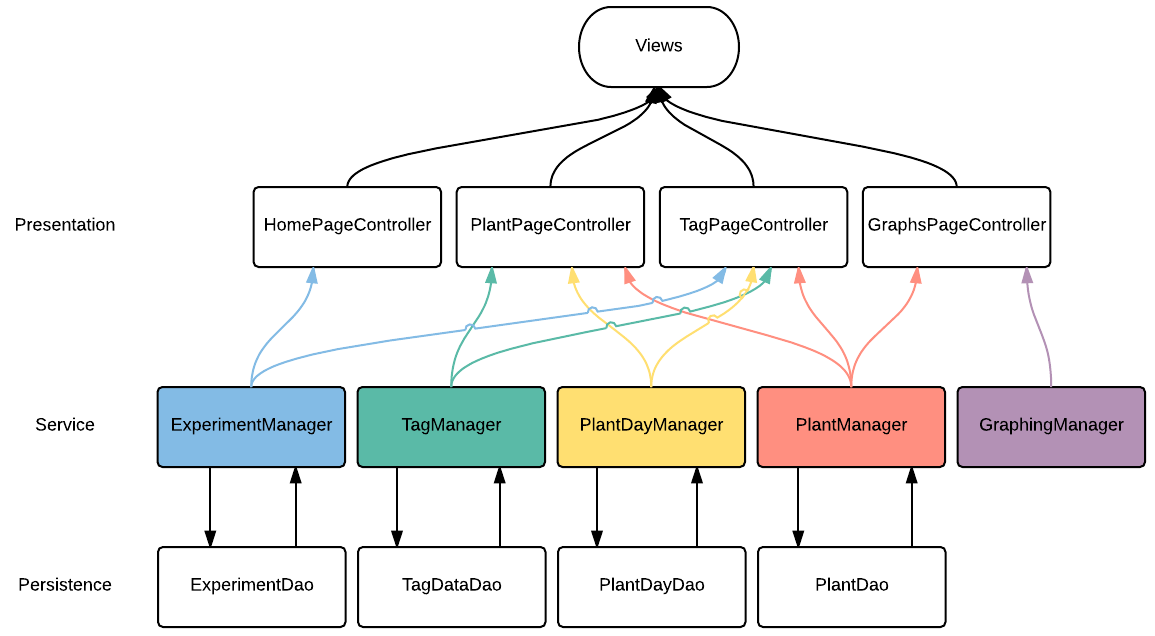
\includegraphics[width=\textwidth]{images/design/arch1}
    \caption{Architecture and dependency wiring}
    \label{fig:arch1}
\end{figure}

\section{Framework and Programming Language}\label{framework}

The sheer range of MVC frameworks available to developers is incredible and the decision of which to use is potentially difficult. It was not within scope to review a large amount of potential choices and to research which were mature, well supported solutions rather than a `flavour of the month' framework. The two main contenders considered for this project were Ruby-on-Rails and the Java based Spring. Both are mature, well supported technologies with a large range of compatible libraries. Both have large and active communities surrounding and supporting them and both have well maintained official documentation. Both share a  `convention over configuration' approach and importantly both are capable of supporting the designs discussed in section~\ref{arch}.

For the purposes of this project, Spring was eventually selected. Specifically the Spring Boot\cite{_boot} bundle which greatly reduces initial configuration time at the start of a project and allows simple integration of complex packages (such as the Spring-Data package discussed in section~\ref{db}) via so called `starter' packages. Even though both frameworks offer inversion of control and dependency injection, the annotation based Spring approach is preferable, especially when coupled with a fully featured IDE capable of understanding the wired dependencies and annotations. 

Using a framework based on Java has some arguable advantages, the fact that Java is compiled provides an extra level of checking during development and provides a quick notification of overlooked errors that may take time to uncover in an interpreted environment such as that provided by Rails. Java has built in security and type-safety providing peace of mind both in guaranteed resolution of variable types and built in access control at the virtual machine level. 





\section{Domain modelling}

Designing a domain model representation for the project was fairly straight forward. It was clear from initial investigations that a simple relationship existed between the primary domain entities that were going to be represented by the system. Essentially, there are Experiments, Experiments have a number of Plants associated with them and these Plants never belong to more than one Experiment at a time. Each Plant then has a number of images associated with it. There is a clear one to many relationship between these entities that is intuitive and can be modelled easily.

Further consideration of this domain model design following some initial implementation led to the inclusion of the PlantDay class in order to better represent the time serried nature of the images and data associated with a Plant. The Plant class now has many PlantDays which has many PlantImages. Each unique date that has images of a Plant is represented as a PlantDay. PlantImages with the same date are grouped together within the same PlantDay. This gave rise to the final design for the relationship between these domain entities, figure~\ref{fig:domain1} shows how this relationship is modelled within the system. 


\begin{figure}[H]
    \centering
    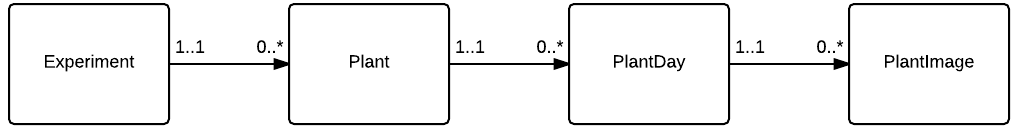
\includegraphics[width=\textwidth]{images/design/domain1}
    \caption{A simplified class diagram showing the relationship between primary domain entities}
    \label{fig:domain1}
\end{figure}


Having modelled the entities in the system, consideration was given to the best approach to adding data to the entities. There are two primary modalities to the data expected within the system, data directly associated with a top-level Plant and time-serried Plant data which would be associated with a date or PlantDay. After investigating different examples of data collected during experiments it was decided that there would be two primary data classes. A Metadata class which would hold a map structure and share a one-to-one relationship with unique Plants and PlantDay instances, and a TagData class which would be unique to the tag content it contained and potentially referenced by many Plant or PlantDay instances.

Since it was clear that experiment data is possibly very different from one experiment to the next, the system had to be permissive in how the data is associated with domain objects. Arbitrary attributes and values had to be supported and this is why the approach with the Metadata class is to have a map structure holding string values for attribute key/value pairs. Using strings meant that both numerical and text data could be represented within the same structure, leaving conversion and/or checking requirements to other parts of the system if required. This was deemed acceptable since for the most part the system is only storing and displaying these data rather than using the values directly for calculations for example. Both the Plant class and PlantDay could have held the metadata map as instance variables, and indeed they did initially, but it became apparent that porting it out into a single class would enable the data to be queried natively on the database (discussed further in section~\ref{db}) and cut down on the number of unique queries required in the Java code in order to find metadata instances.

Whilst the Metadata class represents general experiment data for each Plant and PlantDay, the TagData class was designed to hold sparsely associated data. The majority of Plants would be untagged, tags are used as supplementary comments against the occasional Plant to note some interesting information (common examples seen were `dead' or 'small'). The approach with the TagData class was to have a unique instance for each unique tag, for example, all Plants with the tag `dead' shared a reference to the same tag instance with content `dead'. This provided a simple way to enable returning all Plants sharing a tag within an experiment via queries against the content of the associated TagData. Figure~\ref{fig:domain2} shows the complete relationship between the domain model classes. Essentially these classes are all Plain Old Java Objects (POJO) which is why such a simple diagram suffices, the methods they contain are all getter/setter type methods and can be omitted from the relationship diagrams.


\begin{figure}[H]
    \centering
    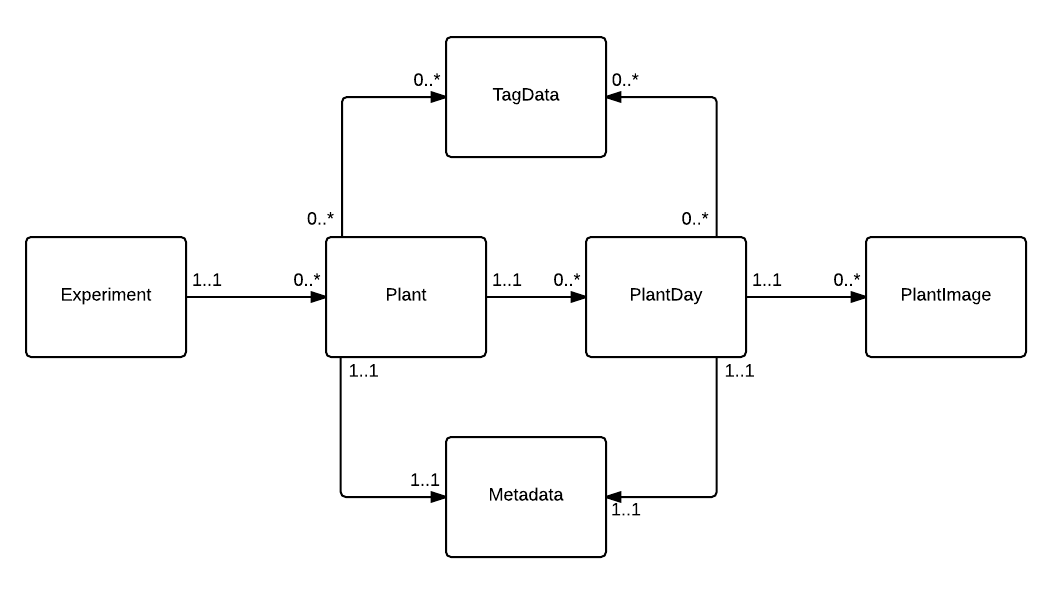
\includegraphics[width=\textwidth]{images/design/domain2}
    \caption{A simplified class diagram showing the domain model}
    \label{fig:domain2}
\end{figure} 

\section{Database} \label{db}

For this project the database structure is entirely derived by the Hibernate\cite{_hibernate} object relational mapping (ORM) which is included in the Spring framework within the Spring-Data project as part of its Java Persistence API (JPA) support. The ORM system allows a developer to annotate Java code with keywords that inform the ORM system of how to represent a given class and persist it in the database. This technique allows the developer to manage the persistence element of a system from within the same object-oriented paradigm that the rest of the system is written in. It provides a level of abstraction away from the managing of the database itself leaving the developer to define only the structure of the data rather than its precise representation within a specific database system.

 Listing~\ref{lst:orm} shows an example of these annotations within the Plant class. The class is annotated with \texttt{@Entity} to inform the ORM that it is a managed class to be persisted and table constraints are declared. The getter methods for the instance variables in the class are annotated with relationship definitions if applicable, including foreign key mappings and what manner of database instructions should cascade through the relationship to the related entity. The annotations can also define a fetch type which can take the value \texttt{LAZY} or \texttt{EAGER}, this defines whether the related entity objects should be fully initialised when the parent is called or whether, in the case of a \texttt{LAZY} fetch, a proxy object with no instance variables initialised should be returned. For this project, the use of \texttt{LAZY} fetch is preferred in all situations since it allows greater control over the performance of the system. If for example, the Plant class made an eager fetch for it's associated list of PlantDay objects, each PlantDay would be fully initialised at the time when the Plant object is retrieved from the database via a query, resulting in extra queries to the database in order to fully populate each PlantDay. Using this fetch technique allowed the PlantDays to be initialised when a method like \texttt{.size()} was invoked on their containing list or a getter method was invoked on the PlantDay itself. 

\lstjava
\lstinputlisting[label={lst:orm},caption=Detail of ORM annotation in Java class]{sourceCode/mySnippets/design/plantorm.java}

Figure~\ref{fig:dbSchema} details the database schema resulting from the ORM annotated relationships within the system. As discussed previously in this section, the relationships are a direct result of the structure of the Java code and the choices made with certain annotations, such as which side of a relation should hold a reference to the other.

 The main deliberate change made to the default ORM mapping onto the database was to pull the dataAttributes map (a \texttt{Map<String,String>} representation in Java) out from the Metadata object into its own table, `metadata\_data\_attributes'. The default would have been to map this as a blob type column within the metadata table, however, in order to ensure that all data within the database can be queried via native queries on the database itself, this extra table approach was taken.


\begin{figure}[H]
    \centering
    \includegraphics[width=\textwidth]{images/design/dbSchema}
    \caption{An entity relationship diagram for the database schema}
    \label{fig:dbSchema}
\end{figure}

From a developer based standpoint, when using an ORM such as the Hibernate system provided in Spring, the underlying database technology is mostly transparent. Provided the database is of a type supported by the ORM, the developer need not make any changes to the code in the system in order for the underlying database technology to change. Custom queries implemented within the system are defined using JPA syntax and are abstracted away from the underlying database. However, consideration was given to the database system to ensure that the best choice was made both to support efficient representation and to ensure compatibility with a wide range of possible hosting environments and potential future maintenance needs.

It was clear from very early in the project that the data to be persisted within the system had structured relationships between entities which favours the more traditional SQL type databases over NoSQL solutions. It is forecast that the increased scalability offered by a NoSQL solution would not be required for this system, traditional SQL management systems are capable of scaling up to many millions of entries which should be more than sufficient for this system. With this in mind a MySQL solution was chosen, it is widely supported and well understood in terms of potential maintainers along with being a default technology on many operating systems including the hosted environment provided for the system.

\section{Data Import}

When designing the data import system the primary objective was to try and preserve, as much as possible, the format and structure of the original data files produced as part of an experiment. Figure~\ref{fig:data1} shows an excerpt from a spreadsheet provided as an example of real experiment data. 

\begin{figure}[H]
    \centering
    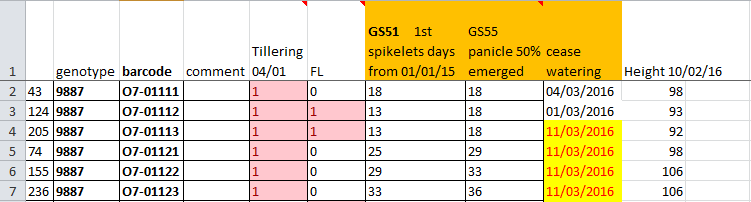
\includegraphics[width=\textwidth]{images/design/data1}
    \caption{A sample of provided experiment data in its original form}
    \label{fig:data1}
\end{figure}

For representing these data, the CSV format is the obvious choice and is available as one of the default export options for spreadsheet applications. The design challenge was routing the data from the CSV file into the system whilst enabling arbitrary values for identifiers to allow for the vast potential range of different data to be captured by the system. However, the format of the files needed to change as little as possible to simplify the use of the system and to minimise the amount of work required on the data to get it ready for import.

The solution was to use a simple annotation based method to identify how each column of the CSV should be routed. Listing~\ref{lst:annot} shows how these annotations are represented and used within the header of the csv file. 
\begin{lstlisting}[label={lst:annot},caption=Excerpt showing annotated CSV header for data import]
{{plant-a}}genotype,{{bc}}barcode, {{plant-t}}comment,{{day-a}}Growth Stage~~51,
\end{lstlisting}
There are four supported annotations:
\begin{enumerate}
\item \textbf{\{\{bc\}\}} - Identifies the column as the barcode for a Plant. This serves to uniquely identify the Plant to which the data in the row should be assigned.
\item \textbf{\{\{plant-a\}\}} - Identifies the column as a Plant attribute. The content of the header column is used as the identifier and the content within the row is used as value. 
\item \textbf{\{\{plant-t\}\}} - Identifies the column as a Plant tag. The content of the header column is ignored and the content of the row is added as TagData to a Plant.
\item \textbf{\{\{day-a\}\}} - Identifies the column as a PlantDay attribute. Uses a specific delimiter token \verb|~~| in order to split the header column into a key value pair. The column in the row in this instance needs to be a date such that a specific day can be allocated the data.
\end{enumerate}

Other methods investigated included using XML and JSON within the CSV to identify certain fields in the header and columns. However, even though both XML and JSON are convenient ways to represent and parse semi-structured data, they are not particularly quick to use in terms of the characters needed to be typed and neither are they especially readable when crammed into the header of a CSV file. In keeping with the goal of simplicity these alternatives were quickly discounted in favour of the simple annotation method. 

\section{UI}
The UI design process used within the project is fairly straight forward and relatively basic. Essentially the process used would first involve a wire frame mock up of the page, an example for the Plant Detail page is shown in figure~\ref{fig:ui1}. This would then be prototyped and the design would evolve iteratively as implementation proceeded and user feedback testing was conducted.

\begin{figure}[H]
    \centering
    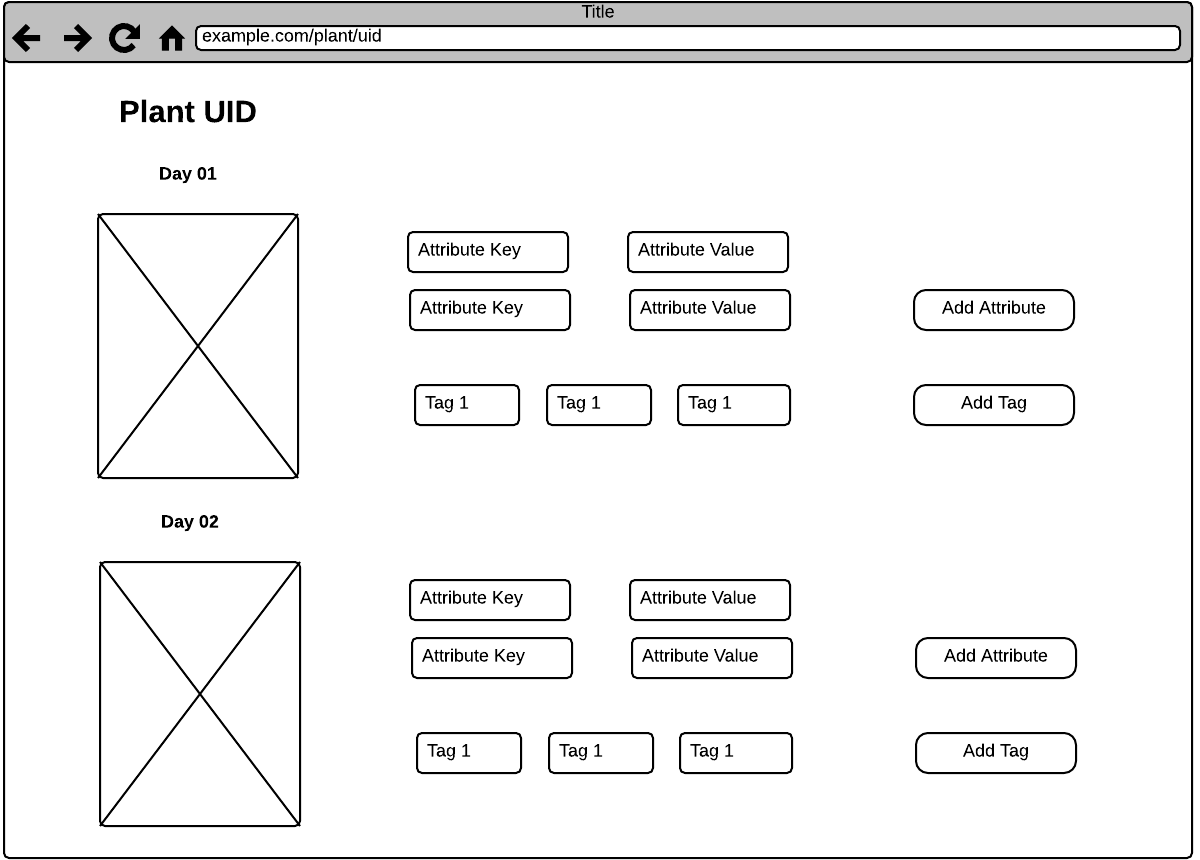
\includegraphics[width=\textwidth]{images/design/ui1}
    \caption{An early wireframe design for the Plant Details page}
    \label{fig:ui1}
\end{figure}

Figure~\ref{fig:ui2} shows the final look of the Plant Detail page, it's clear to see how it relates to the initial wire frame and also where implementation decisions have resulted in some minor tweaks to the design. This same process was followed for all the pages within the system, where the focus has been on a simple yet usable design with minimal clutter. 

\begin{figure}[H]
    \centering
    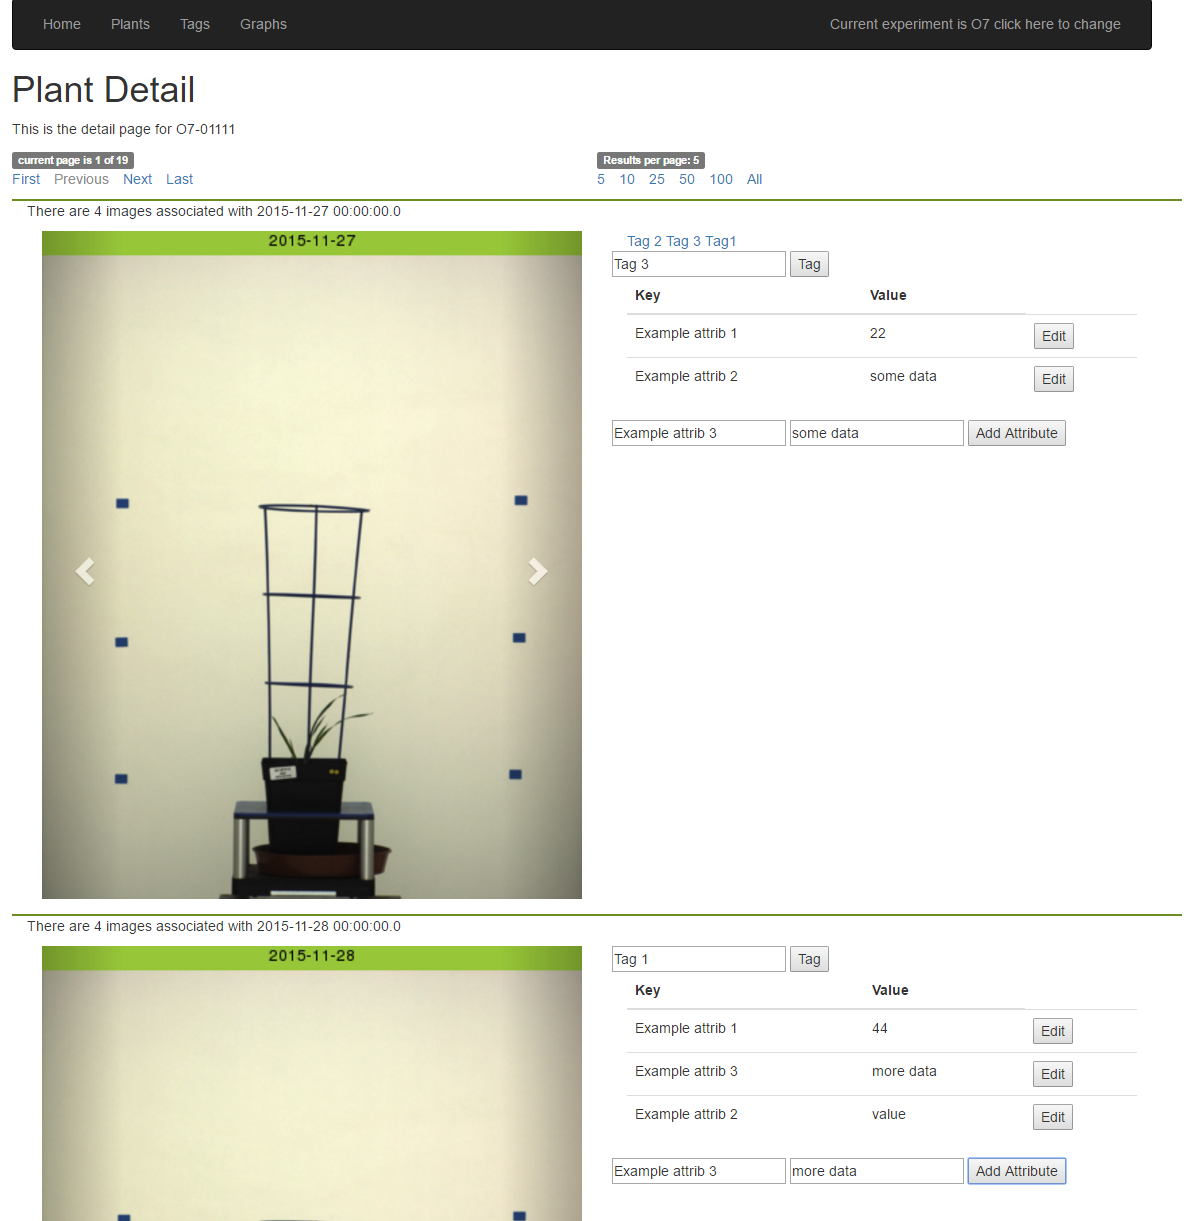
\includegraphics[width=\textwidth]{images/design/ui2}
    \caption{A screen shot showing final design of Plant Details page}
    \label{fig:ui2}
\end{figure}



\section{Tools and third-party services}
\subsection{Intellij}

Intellij \cite{_intellij} is the core development tool used during the completion of this project. It is a fully featured Java integrated development environment (IDE) that has support for a wide range of features including Spring and Github (see section \ref{gitsection}) integration right out of the box. Its code completion and debugging tools are significantly more refined in comparison to the most popular alternative Eclipse, allowing for faster writing of code and easier debugging. As with any reasonably modern IDE, IntelliJ comes with the facility to run sophisticated test suites, providing code coverage metrics and providing auto-generated method stubs in implementation or test classes further speeding up development time, especially in boiler-plate heavy languages such as Java.

IntelliJ also provides in-built static analysis tools that run automatically has part of committing changes to version control via the IDE. This is useful as it is configured to highlight warning level issues which include code style along with potential logical mistakes within sections of code and even spelling errors. Having these checks at commit time enables the developer to review any potential problems before the code gets checked into the repository, although the results are often a little too pessimistic they are still useful. Figure \ref{fig:intellij} shows the IntelliJ IDE with static analysis results displayed.

\begin{figure}[H]
    \centering
    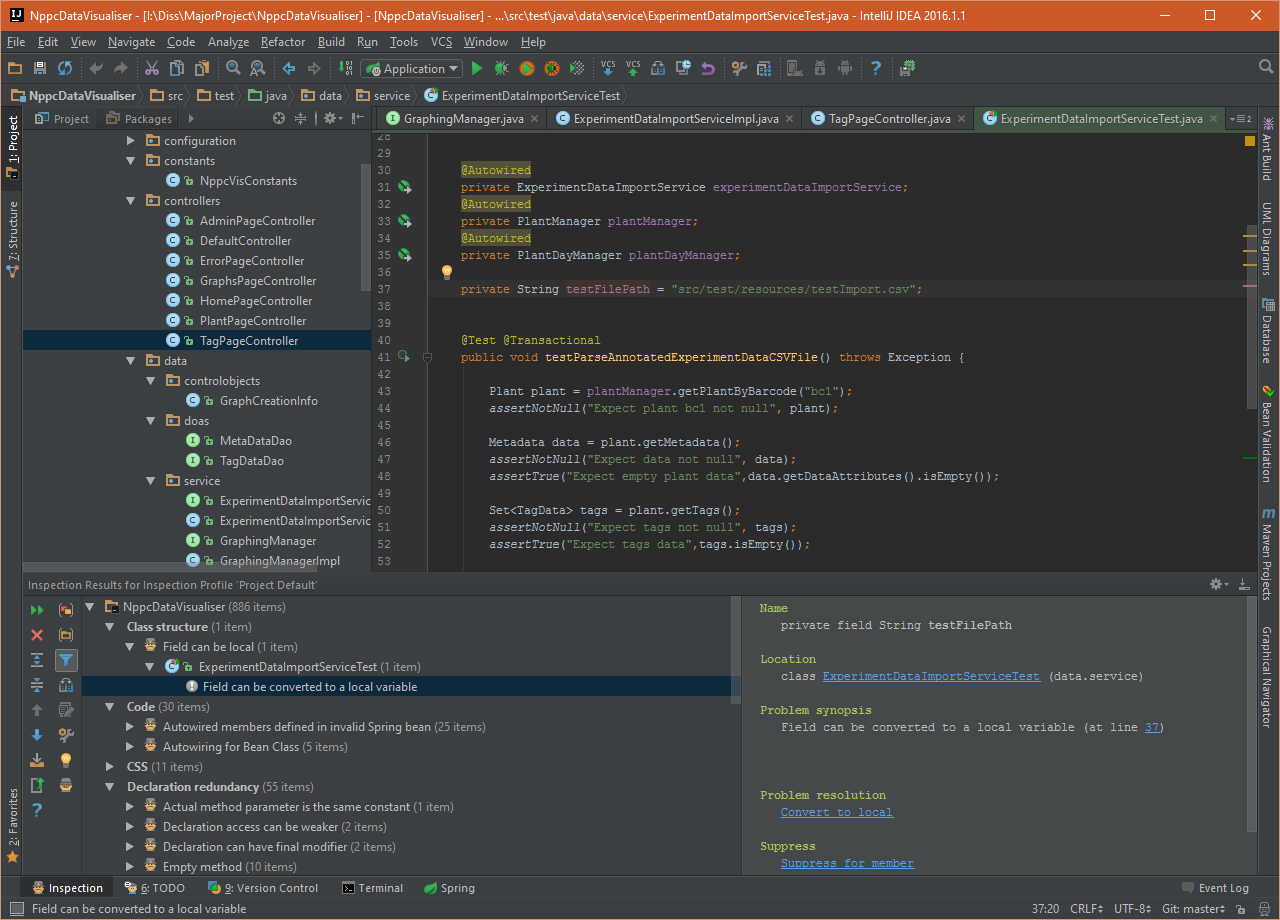
\includegraphics[width=\textwidth]{images/tools/intellij}
    \caption{The IntelliJ IDE showing result of static analysis}
    \label{fig:intellij}
\end{figure}

\subsection{Git and Github} \label{gitsection}

The use of version control is invaluable in modern software development. It has become a necessity in even the smallest of hobby projects since it allows the developer to be confident in making changes without having to worry about rescuing previous version if things go wrong and provides development teams with the means to work concurrently and collaboratively on the same code base. 

The version control system selected for this project was Git \cite{_git}, having previously used alternatives such as Subversion I chose Git for its integration with more numerous, modern services and the fact that it allows local copies of a repository which is synced with a remote repository as opposed to the remote-only approach taken by Subversion.

The Git repository for this project is hosted on Github \cite{_gitHub}, a web based service dedicated to providing git repository hosting and related facilities, such as commit history tracking, release visioning and integration with third party services. There are alternatives to Github available but due to familiarity brought on by hosting all previous projects and the fact that Github is now an industry leading solution, it was decided to use Github for this project without any real evaluation of alternatives since it was well known that Github could provide all facilities required for the purpose of this project. Figure \ref{fig:gitrel} details one of the tagged release versions of the system within Github. Having releases tagged in this way allows easy rollbacks to previous release versions in the event of any major issues in a new release. 

\begin{figure}[H]
    \centering
    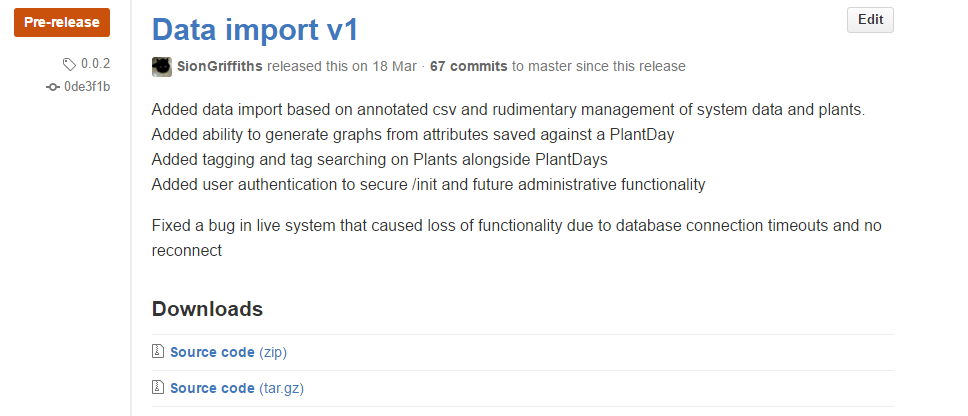
\includegraphics[width=\textwidth]{images/tools/gitrel}
    \caption{A tagged release of the project within Github}
    \label{fig:gitrel}
\end{figure}

\subsection{Jira} \label{jira_sec}

Jira \cite{jira} in an issue tracking and project management tool provided by Atlassian, an Australian software company. It is an industry leading product used by many companies for tracking their projects and the issues within them. Its use on this project was in support of the agile approach to project development, allowing the specification of user stories, development tasks and their inclusions within configurable sprints or development iterations. Figure \ref{fig:jira_sprint} shows the current sprint view in Jira, user stories are grouped into `lanes' corresponding to their status, allowing a simple way to track the work completed and left to do within in the current development iteration.

\begin{figure}[H]
    \centering
    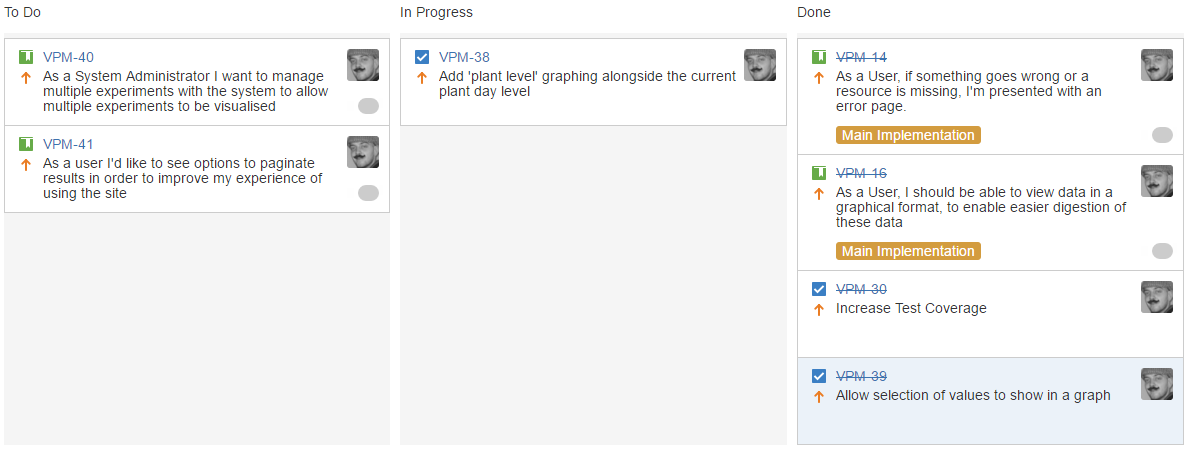
\includegraphics[width=\textwidth]{images/tools/sprint1}
    \caption{Current sprint screen in Jira}
    \label{fig:jira_sprint}
\end{figure} 

 Bugs could also be tracked as issues within Jira and added to the current sprint if necessary, I found this to be a valuable way to deal with emergent issues during development as it allowed a simple way to assign priority to urgent issues and keep track of less usgent bugs in the project backlog to be worked on in a future sprint. Figure \ref{fig:jira_bugs} shows a selection of bugs raised as part of development, Jira provides simple methods for filtering all issues against a project by type or status allowing quick access to screens such as this.

\begin{figure}[H]
    \centering
    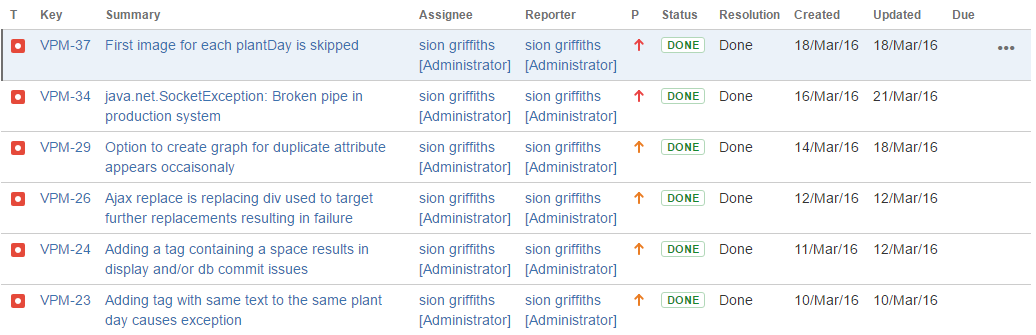
\includegraphics[width=\textwidth]{images/tools/jira_bugs}
    \caption{A sample of bugs raised in Jira}
    \label{fig:jira_bugs}
\end{figure} 

Another helpful feature was the integration with the version control repository hosted on Github. Referencing the issue ID in Jira in a commit message linked the commits with the issue within Jira. This provided a handy way to track development against particular issues over time and allowed a quick way to navigate between the issues in Jira and the commits on Github. 

\begin{figure}[H]
    \centering
    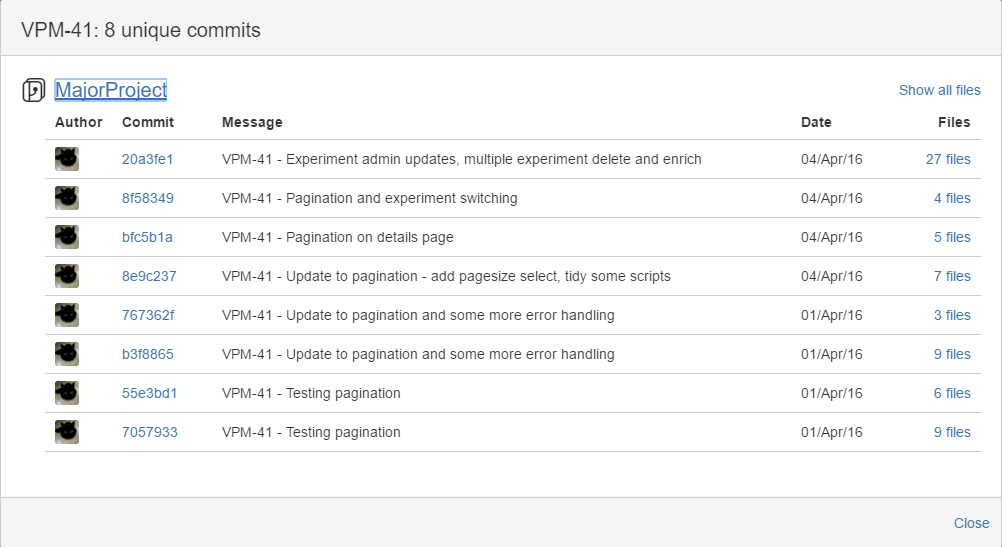
\includegraphics[width=\textwidth]{images/tools/jira_commit}
    \caption{The version control commit tracking within Jira}
    \label{fig:jira_commit}
\end{figure} 

There are a vast array of alternatives that could have been used for issue tracking within the project, many provide the full array of features that were used in Jira during the development of this project. However, Jira being the industry leader, provided an opportunity to gain further valuable experience of its use in a day to day, agile development project. Having previously been involved in the running of a Jira system during my time in industry provided me with familiarisation in configuring a project for my needs and confidence in being able to do so quickly. This was enough to chose Jira over the alternatives that were evaluated such as Waffle.io and the native issue tracking feature provided with Github.

\subsection{Codeship} 
Codeship\cite{_codeship} is a web based Continuous Integration(CI) service. Working in conjunction with the version control repository, Codeship will detect up any commits made to the repository hosted on Github and execute build and test scripts defined as part of the initial setup of the CI service. Use of a CI system within the project provided assurance that each incremental change made to the system integrated correctly and that all tests continued to pass. A notification would be sent in the event of build or test failure.  

 The build script for the project can be seen in figure~\ref{fig:build_script} showing how the project databases are setup and the environment is configured prior to executing the project build and test commands.

 The scripts are invoked within small Docker \cite{docker} based environments which allow build dependencies to be modularised and configured quickly. The initial integration of the CI system into the project environment was extremely simple, linking the Github repository for the project was a couple of mouse clicks and the script below is the entirety of the extra configuration required to get the CI system fully up and running. It was because of this speed and simplicity of configuration that Codeship was chosen over rival offerings such as TravisCI \cite{travis} which appeared to have a much more complex initial setup during evaluation.

\begin{figure}[H]
    \centering
    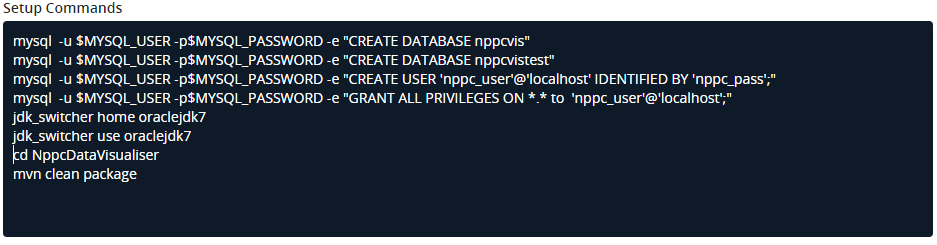
\includegraphics[width=\textwidth]{images/tools/codeShipScript}
    \caption{The project build script on Codeship}
    \label{fig:build_script}
\end{figure} 

\begin{figure}[H]
    \centering
    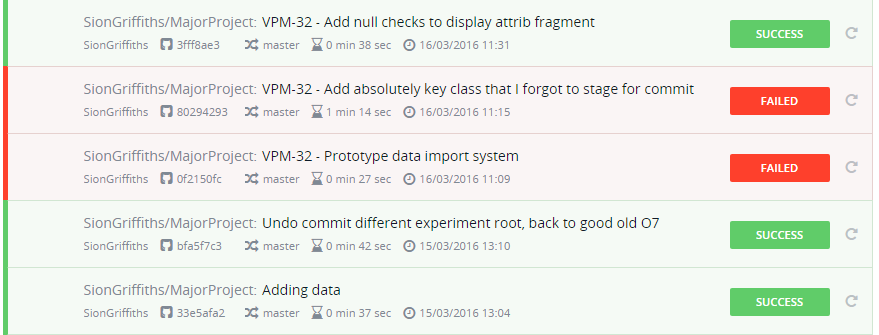
\includegraphics[width=\textwidth]{images/tools/codeShipSmall}
    \caption{A sample of the build history in Codeship}
    \label{fig:build_history}
\end{figure} 



\subsection{Plotly.js}

Plotly.js\cite{_plotly} is an open source graphing library built on top of technologies such as d3.js, a Javascript data manipulation and visualisation library, and stack.gl, a wrapper around WebGL and other associated technologies. There are numerous alternatives libraries that could have been chosen, including d3.js itself and Google Charts amongst others, but the ease of integration with the system and the look and feel of the output from Plotly.js made it the superior choice for this project. Figure~\ref{fig:plotly} shows a Plotly.js generated graph embedded within the Graphs page in the system.


\begin{figure}[H]
    \centering
    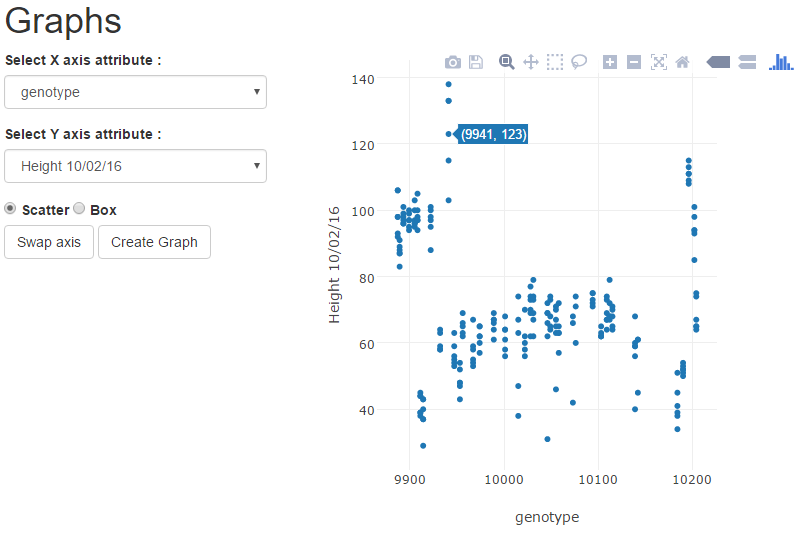
\includegraphics[width=\textwidth]{images/design/plotly}
    \caption{Project graph page featuring a Plotly.js generated graph}
    \label{fig:plotly}
\end{figure} 
